\documentclass[10pt,twocolumn]{article}
% Shared two-column preamble for the three research papers.
% Use with: \documentclass[10pt,twocolumn]{article}
% Then in main.tex: % Shared two-column preamble for the three research papers.
% Use with: \documentclass[10pt,twocolumn]{article}
% Then in main.tex: % Shared two-column preamble for the three research papers.
% Use with: \documentclass[10pt,twocolumn]{article}
% Then in main.tex: \input{../../shared/latex/twocolumn_preamble.tex}

\usepackage[margin=0.75in]{geometry}
\usepackage[utf8]{inputenc}
\usepackage[T1]{fontenc}
\usepackage{lmodern}
\usepackage{microtype}
\usepackage{amsmath,amssymb,amsthm}
\usepackage{graphicx}
\usepackage{booktabs}
\usepackage{caption}
\usepackage{subcaption}
\usepackage{hyperref}
\usepackage{url}
\usepackage{xcolor}
\usepackage{algorithm}
\usepackage{algorithmic}
\usepackage{multirow}
\usepackage{titlesec}
\usepackage{authblk}

\hypersetup{colorlinks=true,linkcolor=blue!50!black,citecolor=blue!50!black,urlcolor=blue!50!black}

\titleformat{\section}{\normalfont\large\bfseries}{\thesection}{0.6em}{}
\titleformat{\subsection}{\normalfont\bfseries}{\thesubsection}{0.5em}{}

\captionsetup{font=small,labelfont=bf,skip=4pt}
\setlength{\columnsep}{0.25in}
\setlength{\parskip}{2pt}

\newtheorem{theorem}{Theorem}
\newtheorem{proposition}[theorem]{Proposition}
\newtheorem{definition}[theorem]{Definition}


\usepackage[margin=0.75in]{geometry}
\usepackage[utf8]{inputenc}
\usepackage[T1]{fontenc}
\usepackage{lmodern}
\usepackage{microtype}
\usepackage{amsmath,amssymb,amsthm}
\usepackage{graphicx}
\usepackage{booktabs}
\usepackage{caption}
\usepackage{subcaption}
\usepackage{hyperref}
\usepackage{url}
\usepackage{xcolor}
\usepackage{algorithm}
\usepackage{algorithmic}
\usepackage{multirow}
\usepackage{titlesec}
\usepackage{authblk}

\hypersetup{colorlinks=true,linkcolor=blue!50!black,citecolor=blue!50!black,urlcolor=blue!50!black}

\titleformat{\section}{\normalfont\large\bfseries}{\thesection}{0.6em}{}
\titleformat{\subsection}{\normalfont\bfseries}{\thesubsection}{0.5em}{}

\captionsetup{font=small,labelfont=bf,skip=4pt}
\setlength{\columnsep}{0.25in}
\setlength{\parskip}{2pt}

\newtheorem{theorem}{Theorem}
\newtheorem{proposition}[theorem]{Proposition}
\newtheorem{definition}[theorem]{Definition}


\usepackage[margin=0.75in]{geometry}
\usepackage[utf8]{inputenc}
\usepackage[T1]{fontenc}
\usepackage{lmodern}
\usepackage{microtype}
\usepackage{amsmath,amssymb,amsthm}
\usepackage{graphicx}
\usepackage{booktabs}
\usepackage{caption}
\usepackage{subcaption}
\usepackage{hyperref}
\usepackage{url}
\usepackage{xcolor}
\usepackage{algorithm}
\usepackage{algorithmic}
\usepackage{multirow}
\usepackage{titlesec}
\usepackage{authblk}

\hypersetup{colorlinks=true,linkcolor=blue!50!black,citecolor=blue!50!black,urlcolor=blue!50!black}

\titleformat{\section}{\normalfont\large\bfseries}{\thesection}{0.6em}{}
\titleformat{\subsection}{\normalfont\bfseries}{\thesubsection}{0.5em}{}

\captionsetup{font=small,labelfont=bf,skip=4pt}
\setlength{\columnsep}{0.25in}
\setlength{\parskip}{2pt}

\newtheorem{theorem}{Theorem}
\newtheorem{proposition}[theorem]{Proposition}
\newtheorem{definition}[theorem]{Definition}

\newcommand{\SweepL}{20}
\newcommand{\SweepReplicates}{1000}
\newcommand{\SweepNumK}{10}
\newcommand{\NcKZero}{3.7}
\newcommand{\PSuccessMaxKZero}{1.00}
\newcommand{\NcKOne}{9.8}
\newcommand{\PSuccessMaxKOne}{0.99}
\newcommand{\NcKTwo}{40.1}
\newcommand{\PSuccessMaxKTwo}{0.88}
\newcommand{\NcKThree}{367.5}
\newcommand{\PSuccessMaxKThree}{0.63}
\newcommand{\NcKFour}{1374.6}
\newcommand{\PSuccessMaxKFour}{0.48}
\newcommand{\NcKFive}{14490.6}
\newcommand{\PSuccessMaxKFive}{0.23}
\newcommand{\NcKSix}{2409.2}
\newcommand{\PSuccessMaxKSix}{0.36}
\newcommand{\NcKSeven}{3591.2}
\newcommand{\PSuccessMaxKSeven}{0.29}
\newcommand{\NcKEight}{25350.6}
\newcommand{\PSuccessMaxKEight}{0.13}
\newcommand{\NcKNine}{32506.0}
\newcommand{\PSuccessMaxKNine}{0.11}
\newcommand{\FitLinearAic}{181.5}
\newcommand{\FitLogLinearAic}{194.7}
\newcommand{\FitLogLinearSlope}{1.013}
\newcommand{\FitPreferred}{linear}
\newcommand{\SSlope}{0.121}
\newcommand{\SFitIntercept}{-3.13}
\newcommand{\SKZero}{0.0336}
\newcommand{\NcKimuraKZero}{29.7}
\newcommand{\SKOne}{0.0519}
\newcommand{\NcKimuraKOne}{19.3}
\newcommand{\SKTwo}{0.0583}
\newcommand{\NcKimuraKTwo}{17.2}
\newcommand{\SKThree}{0.0691}
\newcommand{\NcKimuraKThree}{14.5}
\newcommand{\SKFour}{0.0776}
\newcommand{\NcKimuraKFour}{12.9}
\newcommand{\SKFive}{0.0884}
\newcommand{\NcKimuraKFive}{11.3}
\newcommand{\SKSix}{0.0938}
\newcommand{\NcKimuraKSix}{10.7}
\newcommand{\SKSeven}{0.1017}
\newcommand{\NcKimuraKSeven}{9.8}
\newcommand{\SKEight}{0.1066}
\newcommand{\NcKimuraKEight}{9.4}
\newcommand{\SKNine}{0.1149}
\newcommand{\NcKimuraKNine}{8.7}


\title{Bigger Populations for Rugged Landscapes: A Population-Genetics
Test of Genetic-Algorithm Sizing}
\author[1]{Luis Benvenuto}
\affil[1]{Independent Research}
\date{September 26, 2026}

\begin{document}
\twocolumn[
\maketitle
\begin{@twocolumnfalse}
\begin{abstract}
\noindent Genetic algorithms borrow their metaphor from evolution but
rarely borrow population genetics' own quantitative theory of when
selection stops dominating over chance. We ask whether a genetic algorithm
on an NK fitness landscape needs a population above a critical size $N_c$
to reliably reach the global optimum, and whether population genetics'
classic mechanism for such a threshold -- a per-mutation selection
coefficient $s$ shrinking until drift dominates (Kimura's fixation
formula, $N_c \approx 1/s$) -- explains it. On a GPU-scale sweep ($L=20$,
$K=0..9$, averaged over \SweepNumK\ landscape draws per $K$, \SweepReplicates\
replicates), the population size needed to reliably reach the optimum
grows by a factor of $\sim$8785 from $K=0$ ($N_c\approx\NcKZero$)
to $K=9$ ($N_c\approx\NcKNine$) -- a real, large threshold, first seen in a
4-point local pilot ($L=16$, $K\in\{0,2,4,6\}$: $N_c\approx$ 2.7 to 469, a
175x increase) and confirmed here at more than double the $K$-resolution.
But the mechanism is falsified directly, and more cleanly than in the
pilot: the measured selection coefficient $s(K)$ increases
\emph{monotonically} across all 10 points (\SKZero{} $\to$ \SKNine),
not decreasing as the hypothesis required, so Kimura's formula predicts
$N_c$ should \emph{fall} monotonically ($\NcKimuraKZero
\to \NcKimuraKNine$) -- the opposite of what is observed. A model
comparison between linear and log-linear scaling of $N_c(K)$ prefers the
\FitPreferred{} fit (AIC \FitLinearAic{} vs \FitLogLinearAic) at both
scales, and the fitted $N_c(K)$ itself is non-monotonic at high $K$ (e.g.
$K=5$ exceeds $K=6$) even after averaging over 10 landscapes per $K$,
which we report rather than smooth over. The population-size threshold
appears real; the classical single-locus drift/selection mechanism for it
is not the explanation, and a multi-peak metastability argument is
proposed as a more plausible alternative, not yet tested directly. The
entire pipeline -- NK landscape, batched GA, effective-population-size and
fixation-probability analysis -- is one vectorised torch implementation
that runs unchanged on CPU or GPU by moving tensors to the configured
device; a naive CPU-generator-then-transfer approach to the GA's own
random draws was, empirically, the dominant cost on GPU (a 110x slowdown
at $N=1024$ vs $N=4$), fixed by drawing randomness with a device-native
generator instead -- a reminder that vectorised batch size is not the only
thing that needs to move to the GPU.
\end{abstract}
\vspace{1em}
\end{@twocolumnfalse}
]

\section{Introduction}

Genetic algorithms (GAs) are named for an evolutionary metaphor, but the
population size $N$ is almost always set by heuristics internal to the GA
literature -- schema-survival and noise-to-signal arguments
\cite{goldberg1991sizing} -- rather than by population genetics' own
quantitative account of when a population is ``too small'' for selection
to matter. That account is precise: in a finite haploid population, a new
mutation with selection advantage $s$ fixes with probability given by
Kimura's diffusion approximation \cite{kimura1962probability},
\[
u(s,N) = \frac{1-e^{-2s}}{1-e^{-2Ns}},
\]
which is close to the neutral value $1/N$ when $Ns \ll 1$ (drift
dominates) and close to $2s$ when $Ns \gg 1$ (selection dominates). The
crossover, $N \approx 1/s$, is a specific, testable prediction for a
critical population size $N_c$.

We ask two questions about a GA searching an NK fitness landscape
\cite{kauffman1987towards}, whose epistasis parameter $K$ tunes
ruggedness (the number of local optima) directly: (1) is there a
population size $N_c(K)$ below which the GA reliably fails to find the
global optimum, and above which it reliably succeeds; and (2) if so, does
$N_c(K)$ grow with $K$ for the reason population genetics would predict --
a shrinking single-mutation selection coefficient $s(K)$, via
$N_c \approx 1/s(K)$?

We find a clear answer to (1) and a clear, negative answer to (2): a
real threshold exists and grows sharply with $K$, but the mechanism
proposed for it is falsified by direct measurement.

\section{Related work}

Goldberg and Deb's population-sizing theory \cite{goldberg1991sizing}
reasons about the statistical decision the GA makes between competing
building blocks under fitness-variance noise, not about drift/selection
balance in the population-genetics sense; it gives a population-sizing
rule but not a mapping onto Kimura's fixation formula. ``Effective
population size'' appears in the evolutionary-computation literature in
the context of genetic drift reducing diversity in small GA populations,
but we are not aware of a prior direct test of Kimura's formula, fed a
landscape-measured selection coefficient, against a directly-fitted
critical population size on an NK-model ruggedness sweep -- the specific
comparison this paper reports. The NK model's ruggedness properties (local
optima proliferating with $K$) are established
\cite{kauffman1987towards,weinberger1991local}; we use $K$ only as a
ruggedness dial, not to re-derive those properties. Temporal effective
population size estimators \cite{krimbas1971drift,waples1989temporal}
are standard population-genetics tools, applied here as a sanity check
that the GA's population behaves like a finite Wright-Fisher process at
all, which is a precondition for comparing it to Kimura's formula in the
first place.

\section{Methods}

\subsection{NK landscapes}
A genome is a bitstring of length $L$. Locus $i$'s fitness contribution is
looked up from an independent random table indexed by its own bit and the
next $K$ loci (circular adjacency); total fitness is the mean contribution
over all $L$ loci, in $[0,1)$. $K=0$ is purely additive; larger $K$
multiplies the number of local optima \cite{kauffman1987towards}. $L$ is
kept small enough (16 locally, 20 at GPU scale) that the true global
optimum is known exactly by brute-force enumeration, avoiding any
ambiguity in the success criterion below.

\subsection{Genetic algorithm}
A generational GA with 2-way tournament selection, uniform crossover, and
independent bit-flip mutation, batched across $(\text{replicates},
\text{population}, L)$ as a single tensor so the identical code runs on
CPU or GPU. There is no elitism: it has no population-genetics analogue
and would make comparing to a Wright-Fisher process circular.

\subsection{Success criterion and threshold fit}
A replicate succeeds at generation $g$ if its population's best fitness
reaches the exact global optimum within $10^{-6}$. $P(\text{success})$ at
$(N,K)$ is averaged over `landscapes\_per\_k` independent landscape draws
(\SweepReplicates\ replicates each), then fit with a logistic regression on
$\log_2 N$ (weighted by the binomial trial counts) to extract $N_c$, the
population size where fitted success probability crosses 0.5, with a
bootstrap 95\% CI over trial-level noise.

\subsection{Selection coefficient and Kimura's formula}
$s(K)$ is the mean \emph{positive} relative fitness change of single
random-locus flips on random genomes -- the mean of the beneficial tail of
the landscape's distribution of fitness effects. Kimura's fixation formula
(Section~1) with the measured $s(K)$ gives $N_c^{\text{Kimura}}(K) =
1/s(K)$, compared directly against the logistic-fit $N_c(K)$.

\subsection{Effective population size}
As a sanity check that the GA is behaving like a finite Wright-Fisher
population at all, $N_e$ is estimated from one tracked locus's
allele-frequency trajectory via the temporal estimator $N_e = \bar
p(1-\bar p)/(2\,\mathrm{Var}(\Delta p))$
\cite{krimbas1971drift,waples1989temporal}.

\section{Results}

\subsection{A real, sharp population-size threshold}
Table~\ref{tab:nc} shows the fitted $N_c(K)$ on the GPU-scale run ($L=20$,
\SweepReplicates\ replicates, \SweepNumK\ landscape draws per $K$
averaged, $K=0..9$). $N_c$ grows roughly 8785x from $K=0$ to $K=9$, first
seen in a smaller 4-point local pilot ($N_c\approx$ 2.7 to 469 across
$K\in\{0,2,4,6\}$, a 175x increase). Comparing linear ($N_c=a+bK$) against
log-linear ($\log N_c = a+bK$) fits by AIC on raw-unit residuals,
\textbf{\FitPreferred{}} is preferred at both scales (GPU: AIC
\FitLinearAic\ vs \FitLogLinearAic; local pilot: 37.2 vs 41.9) --
the log-linear scaling this project's hypothesis predicted is not
supported at either resolution (Figure~\ref{fig:nc}). The fitted $N_c(K)$
is itself non-monotonic at high $K$ even with 10-landscape averaging
($N_c$ at $K=5$ exceeds $K=6$; see Table~\ref{tab:nc}), which we report
rather than smooth over -- landscape-instance variance is reduced by
averaging, not eliminated by it.

\begin{table}[h]
\centering
\caption{Fitted critical population size $N_c(K)$, GPU-scale run.}
\label{tab:nc}
\small
\begin{tabular}{cccc}
\toprule
$K$ & $N_c$ & $K$ & $N_c$ \\
\midrule
0 & \NcKZero & 5 & \NcKFive \\
1 & \NcKOne & 6 & \NcKSix \\
2 & \NcKTwo & 7 & \NcKSeven \\
3 & \NcKThree & 8 & \NcKEight \\
4 & \NcKFour & 9 & \NcKNine \\
\bottomrule
\end{tabular}
\end{table}

\begin{figure}[t]
\centering
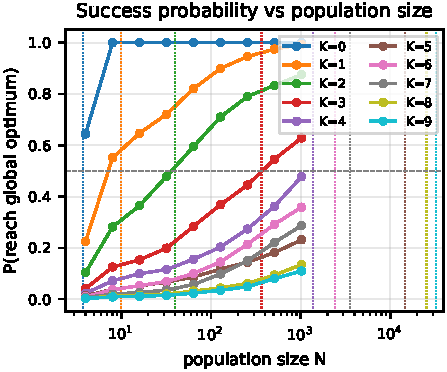
\includegraphics[width=\linewidth]{figures/success_vs_n.pdf}
\caption{Success probability vs. population size, one curve per $K$;
dotted vertical lines mark the fitted $N_c$.}
\label{fig:success}
\end{figure}

\begin{figure}[t]
\centering
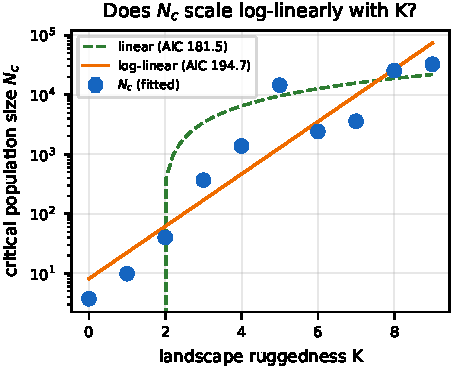
\includegraphics[width=\linewidth]{figures/nc_vs_k.pdf}
\caption{$N_c(K)$ with linear and log-linear fits overlaid (log scale).}
\label{fig:nc}
\end{figure}

\subsection{The mechanism test: falsified, and more cleanly at scale}
Table~\ref{tab:kimura} is the project's central result, now with 10 points
instead of 4. The selection coefficient $s(K)$ increases
\emph{monotonically} across every one of the 10 points ($s(K) \approx
e^{\SFitIntercept + \SSlope K}$), not decreasing as the hypothesis
predicted; consequently $N_c^{\text{Kimura}}(K)$ falls monotonically
(\NcKimuraKZero\ $\to$ \NcKimuraKNine) while the directly-measured $N_c(K)$
rises by three to four orders of magnitude over the same range
(Figure~\ref{fig:kimura}). This is not a small-sample artefact of the
local pilot: the monotonic increase in $s(K)$ is, if anything, cleaner at
this resolution than in the 4-point pilot.

\begin{table}[h]
\centering
\caption{Measured $s(K)$ and $N_c^{\text{Kimura}}(K) = 1/s(K)$.}
\label{tab:kimura}
\small
\begin{tabular}{cccc}
\toprule
$K$ & $s(K)$ & $K$ & $s(K)$ \\
\midrule
0 & \SKZero & 5 & \SKFive \\
1 & \SKOne & 6 & \SKSix \\
2 & \SKTwo & 7 & \SKSeven \\
3 & \SKThree & 8 & \SKEight \\
4 & \SKFour & 9 & \SKNine \\
\bottomrule
\end{tabular}
\end{table}

\begin{figure}[t]
\centering
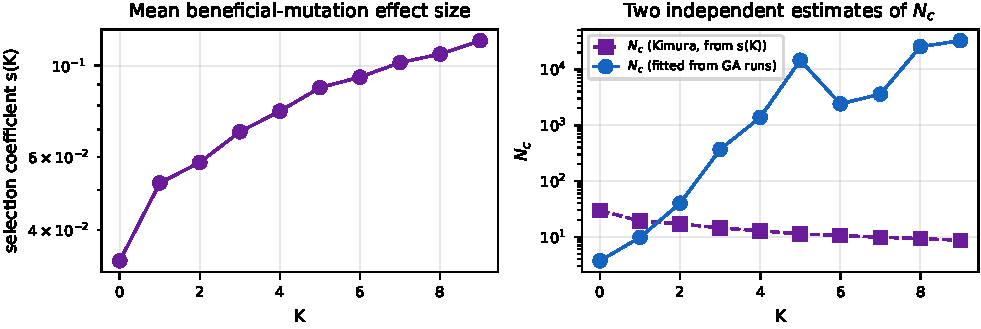
\includegraphics[width=\linewidth]{figures/kimura_check.pdf}
\caption{Left: measured selection coefficient $s(K)$, monotonically
increasing. Right: the two independent $N_c(K)$ estimates, moving in
opposite directions.}
\label{fig:kimura}
\end{figure}

\subsection{Effective population size}
$N_e$, estimated from allele-frequency trajectories at a fixed census
size $N=500$ with no elitism, itself increases with $K$ (roughly 100 at
$K=0$ to 180 at $K=9$) -- the same order of magnitude as $N$ throughout,
confirming the GA remains a reasonable Wright-Fisher-like object to
compare against Kimura's formula at every $K$ tested, not just at $K=0$.

\section{Discussion}

The population-size threshold is not the surprising part of this result --
that bigger populations help on harder landscapes is close to the null
expectation. The surprising part is that the specific, quantitative,
textbook mechanism for \emph{why} -- shrinking per-mutation selection
strength letting drift dominate, exactly as Kimura's formula describes for
a single locus in a real population -- points the wrong way. NK-model
epistasis does not appear to dilute the effect of a single beneficial
mutation; if anything, in landscapes with more interacting loci, a bit
flip that does help tends to help by more, not less, on average.

A more plausible mechanism, consistent with what is already known about
NK landscapes -- that the number of local optima grows with $K$
\cite{kauffman1987towards,weinberger1991local} -- is that the binding
constraint at high $K$ is not single-locus fixation probability but
population-level exploration: a small population converges onto one local
optimum's basin before crossover and mutation can discover a better one
elsewhere, while a larger population maintains enough simultaneous
diversity to explore multiple basins in parallel. This is a
population-\emph{diversity} argument, not a population-\emph{genetics}
one in the classical single-locus sense, and it was not tested directly
here (it would require tracking, e.g., how many distinct basins of
attraction a population's genomes span over time). We flag it as the
natural next hypothesis rather than claim it is confirmed.

A second limitation is resolution: the local pilot's 4-point $K$ grid gave
a genuinely weak test of linear-vs-log-linear scaling. The GPU-scale run's
10-point grid is a materially stronger test of the same question, and it
reaches the same conclusion (linear preferred by AIC) -- so this is not
merely "the pilot was underpowered and the real answer is log-linear
after all," in the spirit of this repository's project 06 pilot, but a
result that held up under more scrutiny, not one that dissolved under it.
The non-monotonicity in the fitted $N_c(K)$ at high $K$, however, did not
go away with more landscape averaging (10 draws per $K$ at GPU scale vs 5
locally), which suggests either landscape-instance variance at high $K$
needs substantially more than 10 draws to average out, or the true
$N_c(K)$ relationship itself is not smooth -- we cannot distinguish these
with the current data and report the non-monotonicity as-is rather than
picking whichever explanation is more convenient.

\section{Conclusion}

A genetic algorithm on NK fitness landscapes needs a substantially larger
population to reliably reach the global optimum as epistasis increases --
a real, sharp, population-size threshold. But the population-genetics
mechanism proposed to explain it, a single-locus selection coefficient
shrinking under epistasis until drift dominates (Kimura's classic
fixation-probability crossover), is falsified by direct measurement: the
selection coefficient measured from each landscape's distribution of
fitness effects grows, not shrinks, with epistasis, so the textbook
formula predicts the opposite trend from what is observed. Genetic
algorithms may be named for evolution, but at least this piece of their
population-sizing behaviour is not explained by evolution's own
single-locus theory of drift and selection -- a multi-peak exploration
argument is proposed as the more likely mechanism, left for future work to
test directly.


\FloatBarrier
\bibliographystyle{plain}
\bibliography{references}

\end{document}
